\documentclass[11pt, a4paper]{article}
\usepackage[affil-it]{authblk} 
\usepackage{etoolbox}
\usepackage{lmodern}
\usepackage{titlesec}
\usepackage{float}

\makeatletter
\patchcmd{\@maketitle}{\LARGE \@title}{\fontsize{20}{19.2}\selectfont\@title}{}{}
\makeatother

\renewcommand\Authfont{\fontsize{16}{14.4}\selectfont}
\renewcommand\Affilfont{\fontsize{12}{10.8}\itshape}

\title{\textbf{Assignment 4}} 
\author{Pavan R Hebbar - 130010046}
\usepackage{graphicx}
\begin{document}
\maketitle
\newpage
\section{Question 1:}

Collision freq of plasma is given by
\begin{equation}
 \nu_{c} = \frac{Ne^4}{16*\pi *\epsilon ^2*m^2*v_{th}^3}
\end{equation}
We get the collison frequency as 0.6
Thus we can consider plasma to be in steady state for time durations of order 10

\section{Question 2:}
Below is the combined velocity distribution plot
\begin{figure}[H]
 \centering
 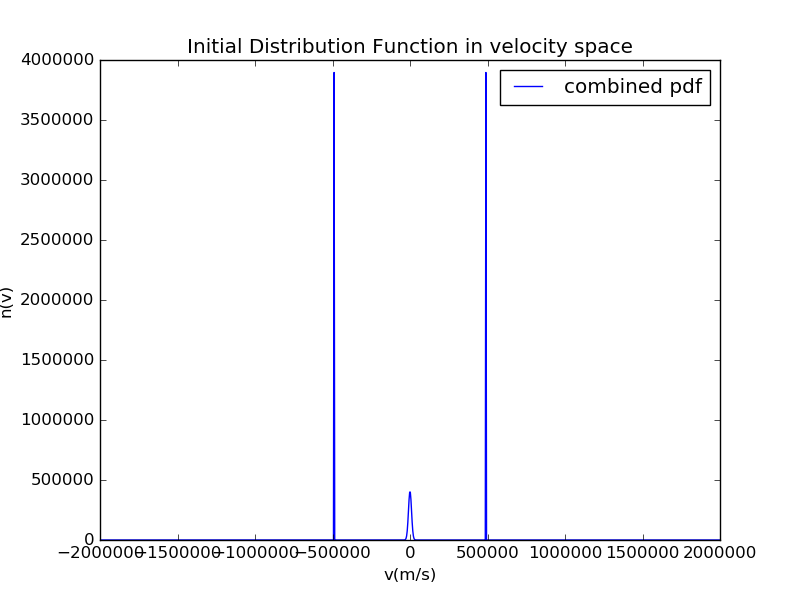
\includegraphics[scale = 0.6]{Init_dist.png}
 \caption{Initial distribution function}
\end{figure}

\section{Question 3:}
Combined density = $3.00*10^10$
Temperature = $1667$eV

\section{Question 4:}
Equilibrium density function is plotted below

\begin{figure}[H]
 \centering
 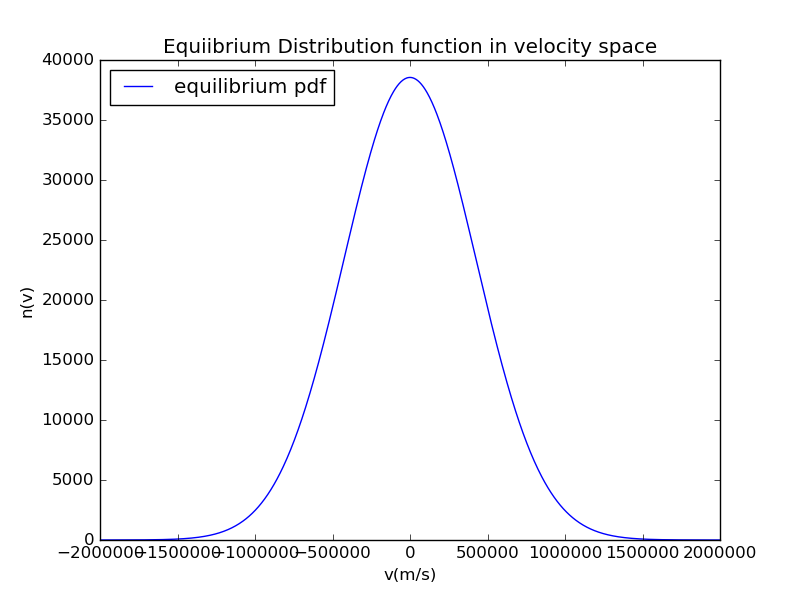
\includegraphics[scale = 0.6]{Eqb_pdf.png}
 \caption{Equilibrium distribution function}
\end{figure}

\section{Question 5:}
(Refer code for simulation) \\
Time taken to reach within 1\% = 1567.21s

\section{Question 6:}
Entropy increases with time. \\
The variation of entropy is plotted below
\begin{figure}[H]
 \centering
 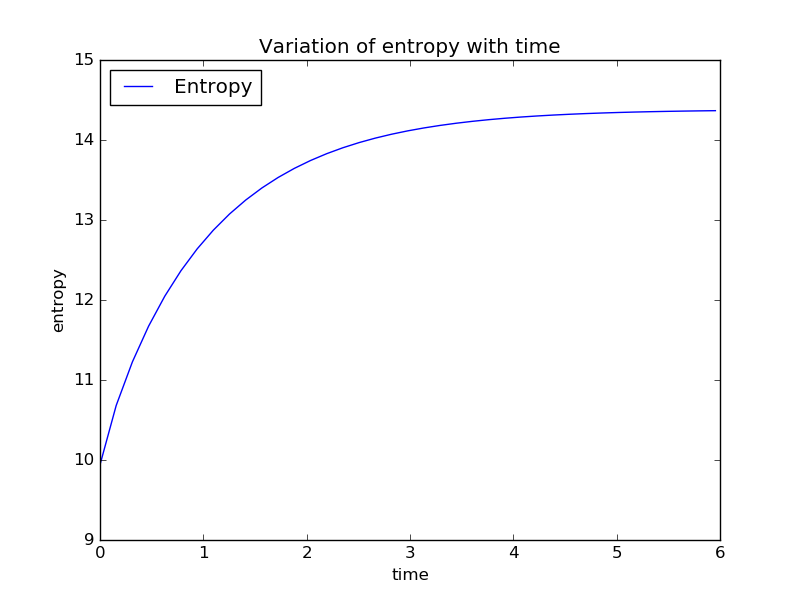
\includegraphics[scale = 0.6]{Entropy.png}
 \caption{Variation of Entropy}
\end{figure}

\end{document}